\chapter{Chargement et netoyage des donn\'ees}

\section{Chargement}
    Tout commence avec la decouverte des donnes. Nous devons alors configurer le
    chargement du fichier CSV, mais avec le choix du separateur (tabulation dans
    notres cas), autorisation des \textit{shortlines}, ...

\section{Types des donn\'ees}
    Nous avions des types parasites dans les donn\'ees. En effet nous
    avions des colonnes considérées comme ``String'' alors qu'elles étaient
    censées être des ``Double''. Ceci est dû à des valeurs parasites (la fameuse
    valeur de latitude ``trolilol'', notamment).

\section{Unicit\'ees des valeurs}
    Nous avions aussi detect\'e des problemes d'unicit\'ees des valeurs. Par
    exemple, il apparaît que l'ID des photos n'est pas unique. Ceci peut être dû
    au fait que la récupération des données se fait en parallèle, et que les
    informations d'une même photo peuvent être récupérées plusieurs fois.
    En partant de l'hypothèse que ces duplicatas représentent les mêmes
    informations, on peut arbitrairement garder un élément par id de photo. Une
    deuxième solution, plus rigoureuse, est de créer un nouvel id garantissant
    l'unicité des informations (càd l'ensemble des colonnes pertinentes: id de
    la photo, id de l'utilisateur, date, tags et légende).

\section{Coh\'erence des donn\'ees}
    Maintenant que nous avions nos matrices bien en forme avec il demeurait un
    souci: la coh\'erence des donn\'ees. Illustrons par un exemple. La colonne
    ann\'ee des donn\'ees est bien un entier, mais il est encore possible que
    l'ann\'ee ait une valeur pouvant alterer les calculs de clustering. Par
    exemple une photo prise en 1780, avant l'invention de l'appareil photo ou
    bien une photo ayant \'et\'e prise dans 10 ans.

    \pagebreak
    \subsection{Ann\'ee de la prise de la photo}
        Ainsi, nous avons decider de filtrer tout les photos aillant ete prise
        avant l'ans 2000 ou dans le futur.

        \begin{figure}[h]
            \centering
            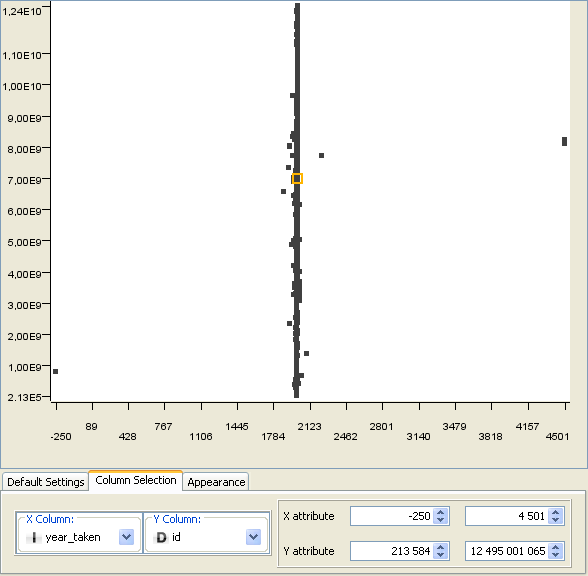
\includegraphics[scale=0.35]{../screenshots/year_id_before.png}
            \caption{Donn\'ees avant filtrage}
            \label{diagram:year_id_before}
        \end{figure}

        \begin{figure}[h]
            \centering
            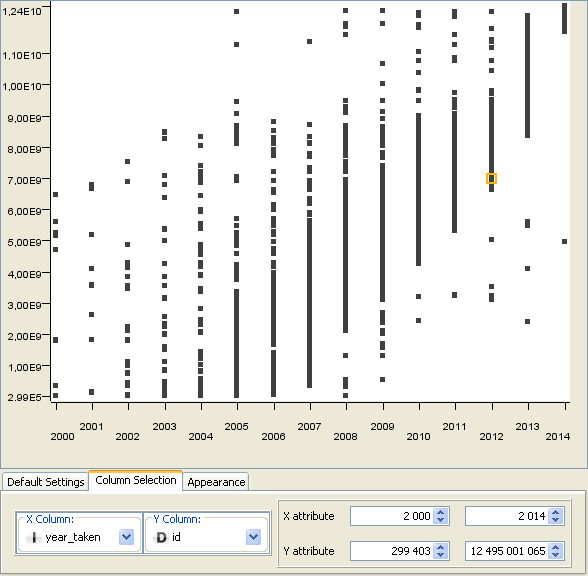
\includegraphics[scale=0.35]{../screenshots/year_id_after.png}
            \caption{Donn\'ees apr\`es filtrage}
            \label{diagram:year_id_after}
        \end{figure}

    \pagebreak
    \subsection{Mois et jour}
        \begin{figure}[h]
            \centering
            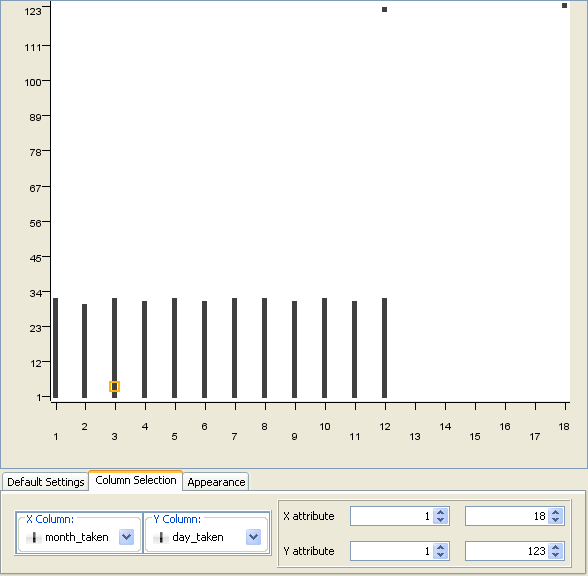
\includegraphics[scale=0.35]{../screenshots/month_day_before.png}
            \caption{Donn\'ees avant filtrage}
            \label{diagram:month_day_before}
        \end{figure}

        \begin{figure}[h]
            \centering
            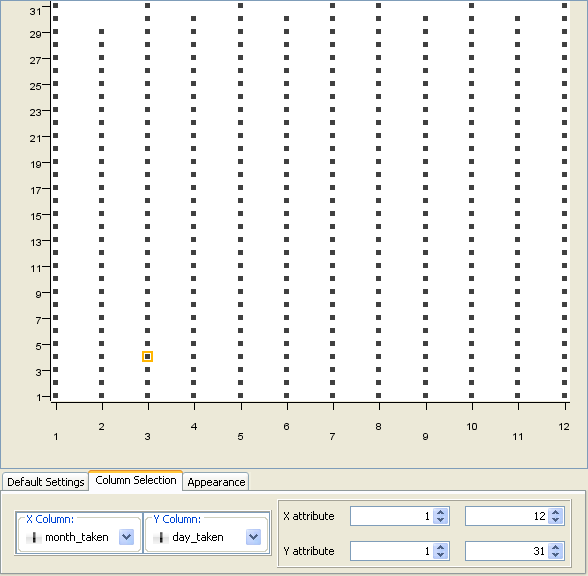
\includegraphics[scale=0.35]{../screenshots/month_day_after.png}
            \caption{Donn\'ees apr\`es filtrage}
            \label{diagram:month_day_after}
        \end{figure}

    \pagebreak
    \subsection{Jour et heure}
        \begin{figure}[h]
            \centering
            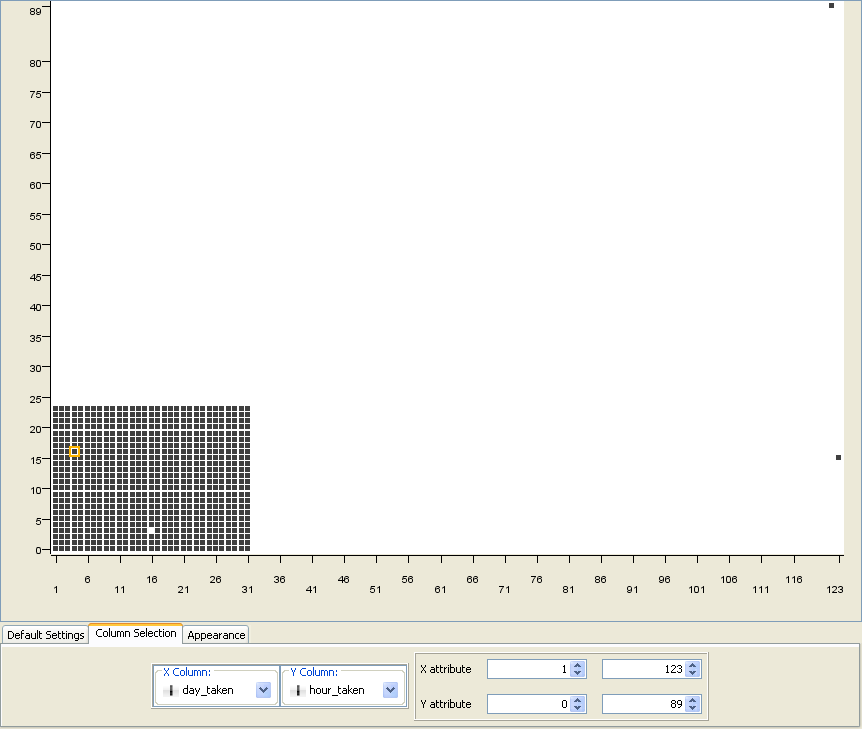
\includegraphics[scale=0.27]{../screenshots/day_hour_before.png}
            \caption{Donn\'ees avant filtrage}
            \label{diagram:day_hour_before}
        \end{figure}

        \begin{figure}[h]
            \centering
            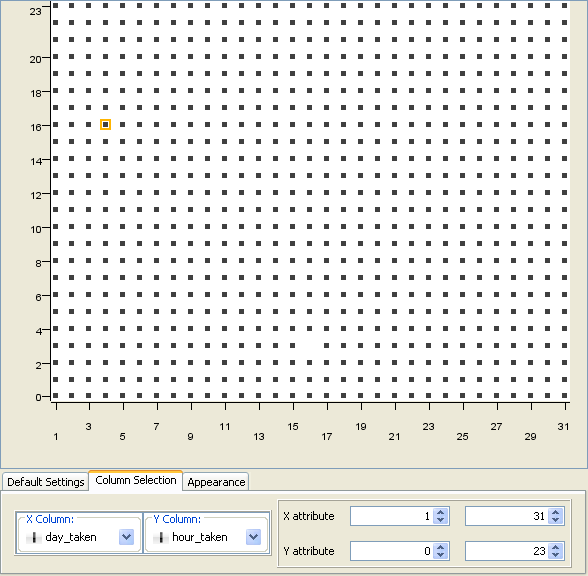
\includegraphics[scale=0.35]{../screenshots/day_hour_after.png}
            \caption{Donn\'ees apr\`es filtrage}
            \label{diagram:day_hour_after}
        \end{figure}

    \pagebreak
    \subsection{Coordonn\'ees GPS}
        \begin{figure}[h]
            \centering
            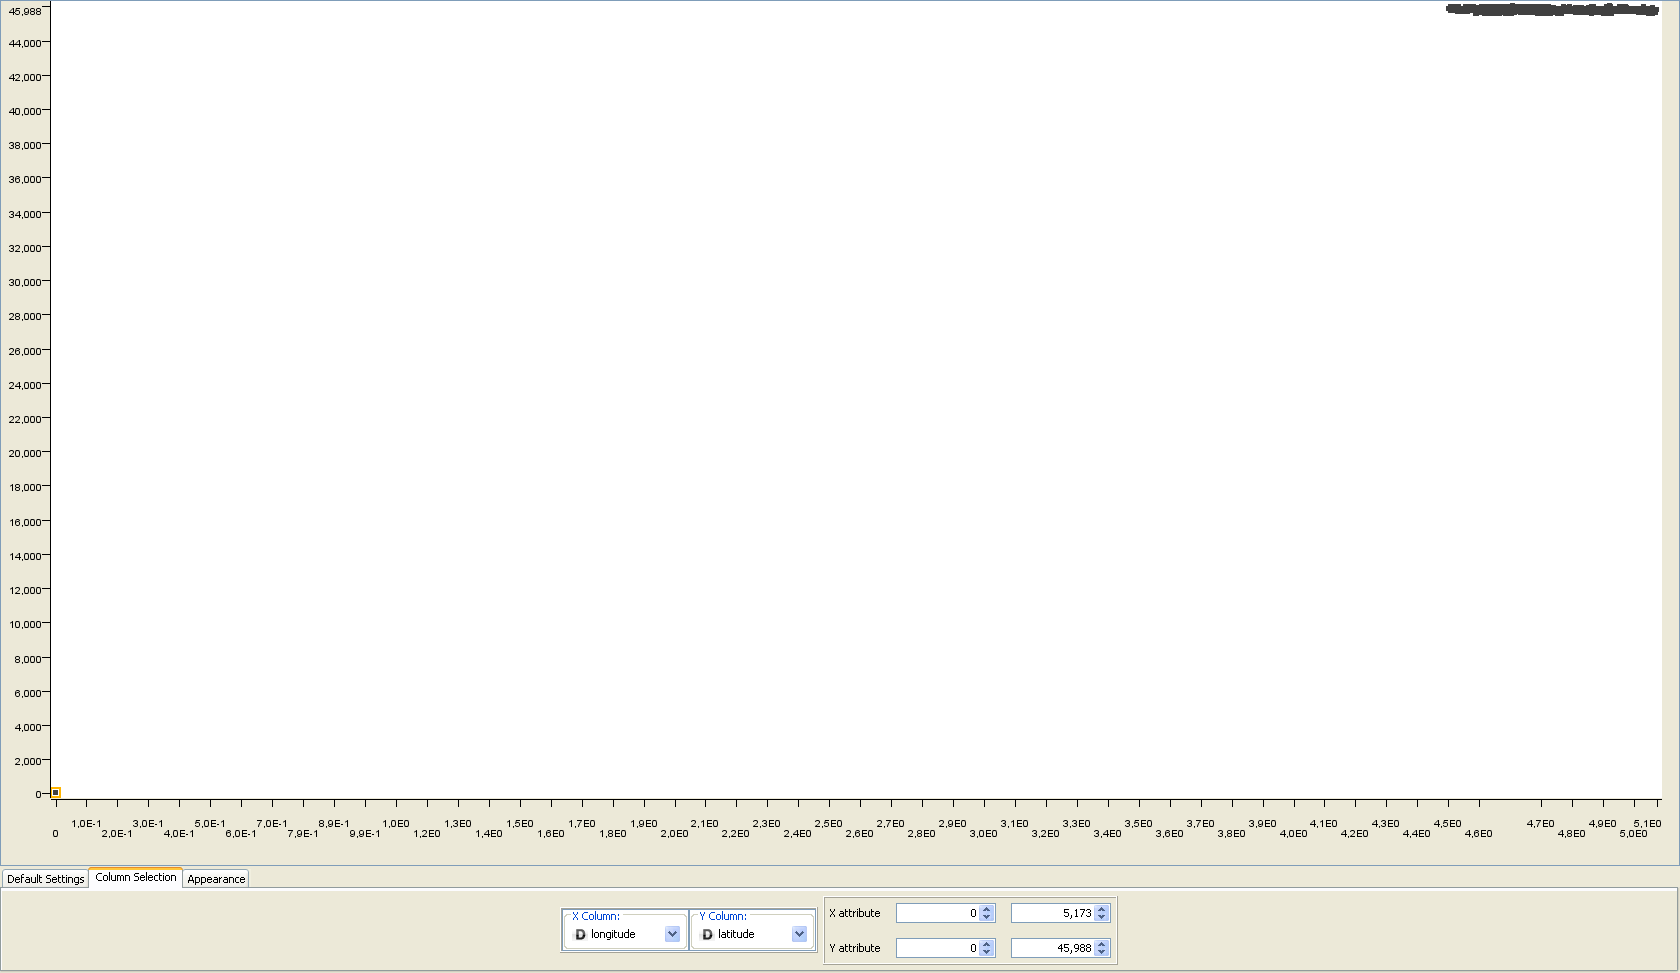
\includegraphics[scale=0.22]{../screenshots/geographic_before.png}
            \caption{Coordonn\'ees GPS avant filtrage}
            \label{diagram:geographic_before}
        \end{figure}

        \begin{figure}[h]
            \centering
            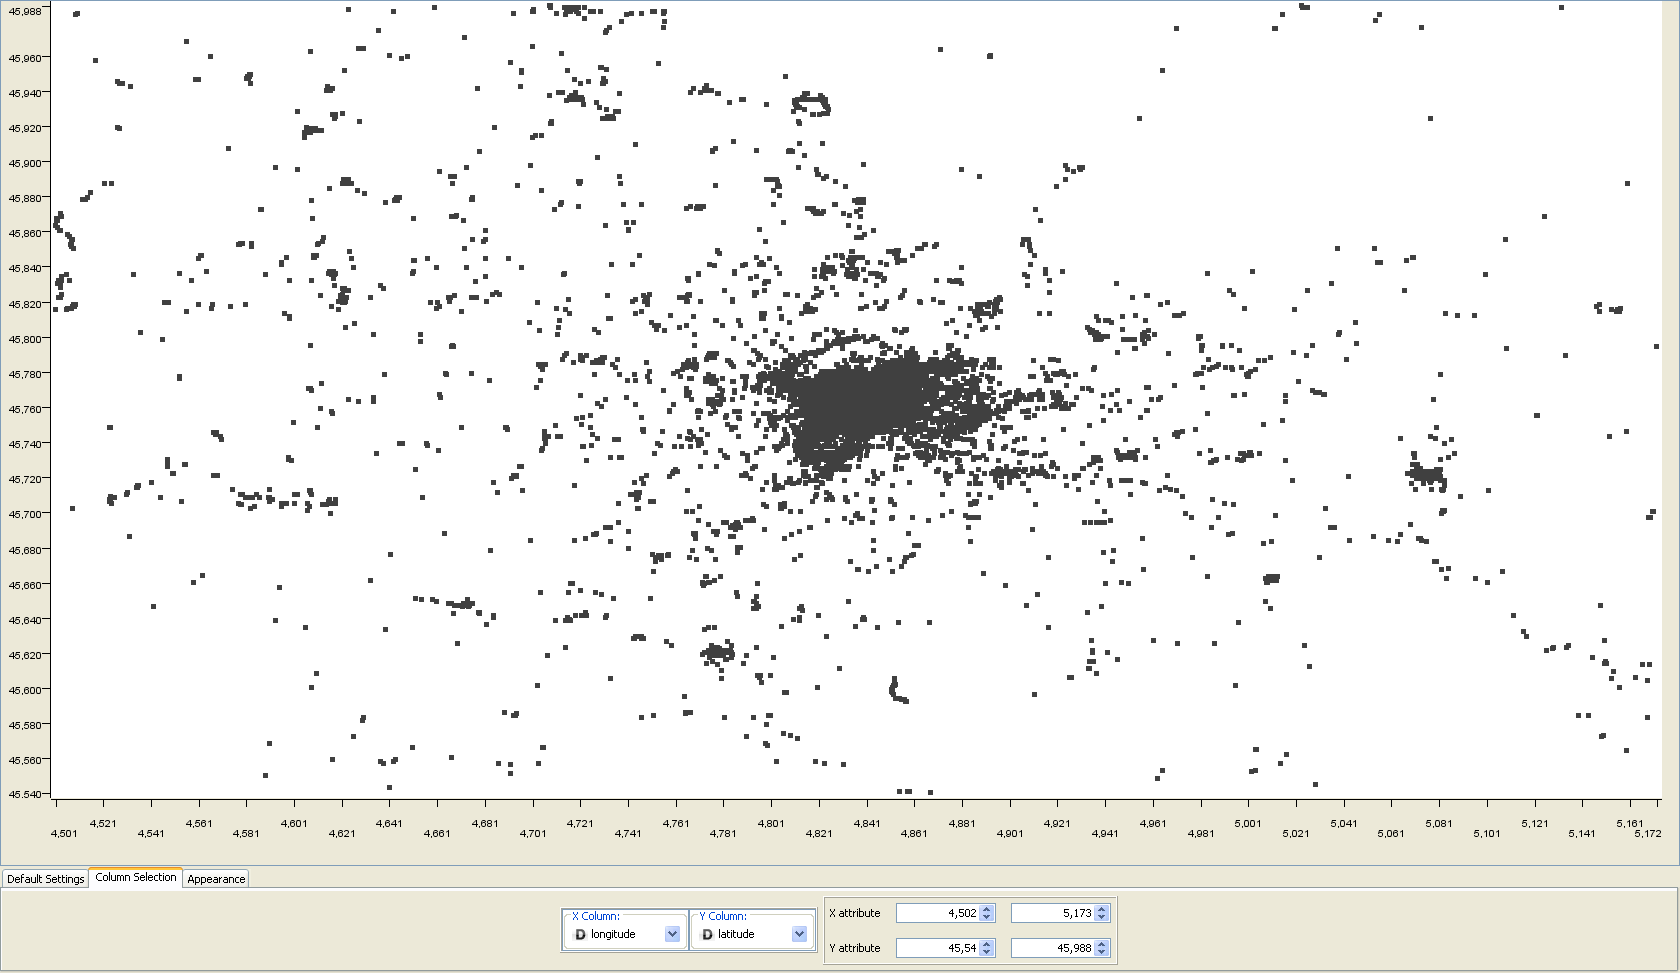
\includegraphics[scale=0.22]{../screenshots/geographic_after.png}
            \caption{Coordonn\'ees GPS apr\`es filtrage}
            \label{diagram:geographic_after}
        \end{figure}
